% v0. 0.10 - 21/03/2024 - added some text about the model and version info
\documentclass[10pt,a4paper]{article}

\usepackage[utf8]{inputenc}
\usepackage[OT4]{fontenc}
\usepackage{amsmath}
\usepackage{amssymb}
\usepackage{graphicx}
\usepackage{fullpage}
\usepackage{hyperref}

\title{Agent-based indoors virus propagation model\\(short description of the sample results)}
\author{Jarosław Miszczak}
\date{21/03/2024 (v. 0.10)}

\begin{document}
\maketitle



%%%%%%%%%%%%%%%%%%%%%%%%%%%%%%%%%%%%%%%%%%%%%%%%%%%%%%%%%%%%%%%%%%%%%%%%%%%%%%%%
\section{Introduction}
%%%%%%%%%%%%%%%%%%%%%%%%%%%%%%%%%%%%%%%%%%%%%%%%%%%%%%%%%%%%%%%%%%%%%%%%%%%%%%%%
This document provides a brief overview of the model for analysing the impact of mobility on the propagation of infections in the indoor environments. We describe few experiments and present the initial results illustrating the models ability.

%%%%%%%%%%%%%%%%%%%%%%%%%%%%%%%%%%%%%%%%%%%%%%%%%%%%%%%%%%%%%%%%%%%%%%%%%%%%%%%%
\section{Agent-based model}
%%%%%%%%%%%%%%%%%%%%%%%%%%%%%%%%%%%%%%%%%%%%%%%%%%%%%%%%%%%%%%%%%%%%%%%%%%%%%%%%

The model was developed using NetLogo language. The source code for the mode is available from \cite{model-src}

\begin{figure}[ht!]
\begin{center}
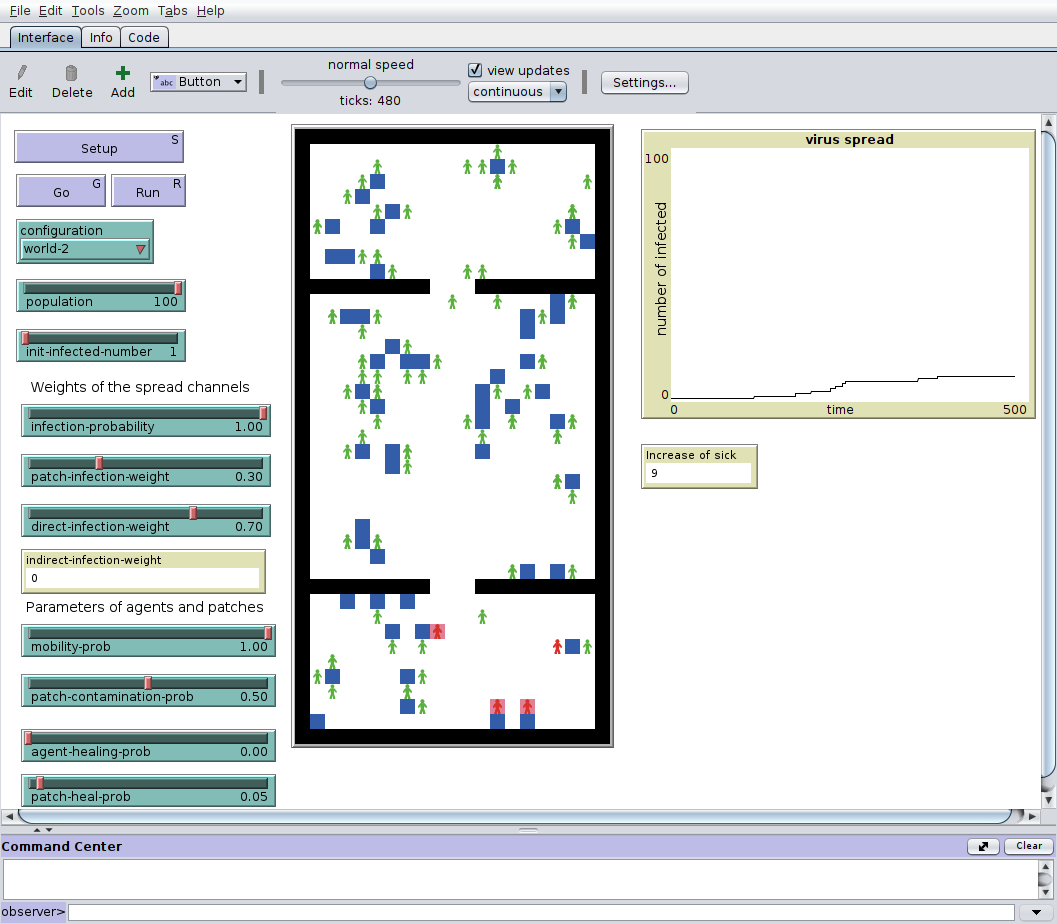
\includegraphics[scale=0.3]{plots/model-gui.png}
\end{center}
\caption{User interface for the NetLogo model of indoors virus propagation with generated configuration. The presented configuration include four modules. Blue patches represent workplaces, and the agents located in their vicinity have decreased mobility. Black patches represent walls.}
\label{fig:gui-world-3}
\end{figure}


%%%%%%%%%%%%%%%%%%%%%%%%%%%%%%%%%%%%%%%%%%%%%%%%%%%%%%%%%%%%%%%%%%%%%%%%%%%%%%%%
\section{Simulation results}
%%%%%%%%%%%%%%%%%%%%%%%%%%%%%%%%%%%%%%%%%%%%%%%%%%%%%%%%%%%%%%%%%%%%%%%%%%%%%%%%

\begin{table}[ht!]
\centering
\begin{tabular}{|c|c|}
\hline
\textbf{Figure} & \textbf{Experiment} \\
\hline
Fig~\ref{fig:sick_increase_large_s_pop100} & exp6  (population 100, world-1)\\
\hline
Fig~\ref{fig:sick_increase_large_s_pop50} & exp6a (population 50, world-1)\\ 
\hline
Fig~\ref{fig:sick_increase_small_s_pop100_world-3} & exp7 (population 100, world-3) \\
\hline
\end{tabular}
\caption{Names of the experiments from \texttt{experiements-v2.xml} file and the the figures with the visualization of the results included in the report.}
\end{table}


\begin{figure}[ht!]
\begin{center}
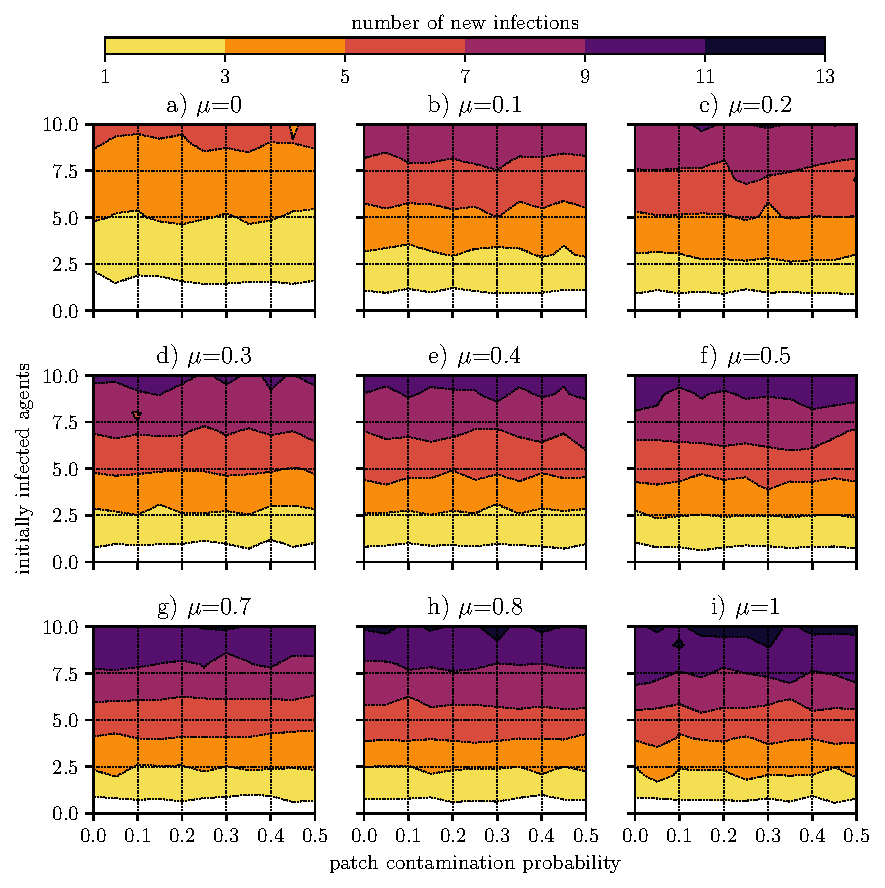
\includegraphics[scale=0.75]{plots/sick_increase_large_s_pop100.pdf}
\end{center}
\caption{Mean increase in the number of infected agents for different values of mobility parameter $\mu$. Each plot represents the absolute increase of the number of infected agents in the population of 100 agents with different number of initially infected agents, ranging from $1$ to $10$,  and with different values of probability contaminating the items.}
\label{fig:sick_increase_large_s_pop100}
\end{figure}


\begin{figure}[ht!]
\begin{center}
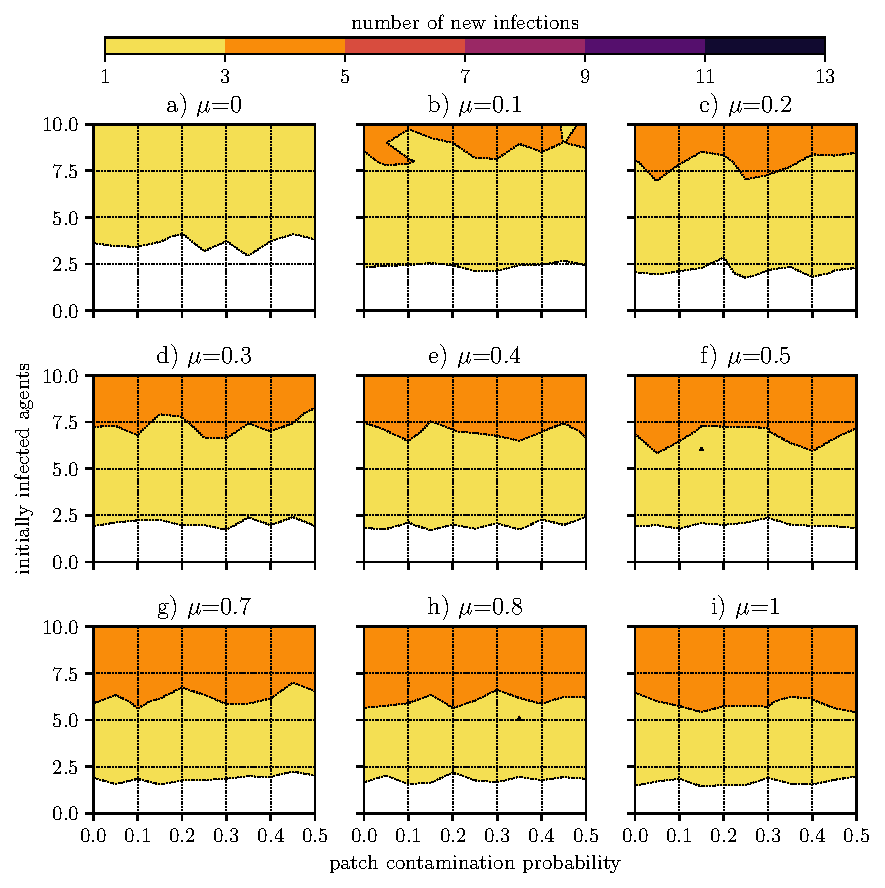
\includegraphics[scale=0.7]{plots/sick_increase_large_s_pop50.pdf}
\end{center}
\caption{Mean increase in the number of infected agents for different values of mobility parameter $\mu$ for the population of 50 agents. Other parameters are described in caption of Fig.~\ref{fig:sick_increase_large_s_pop100} and the colour scale is the same. One should note that even for the significant portion of the infected agents in the population, the spread of the disease is limited.}
\label{fig:sick_increase_large_s_pop50}
\end{figure}



\begin{figure}[ht!]
\begin{center}
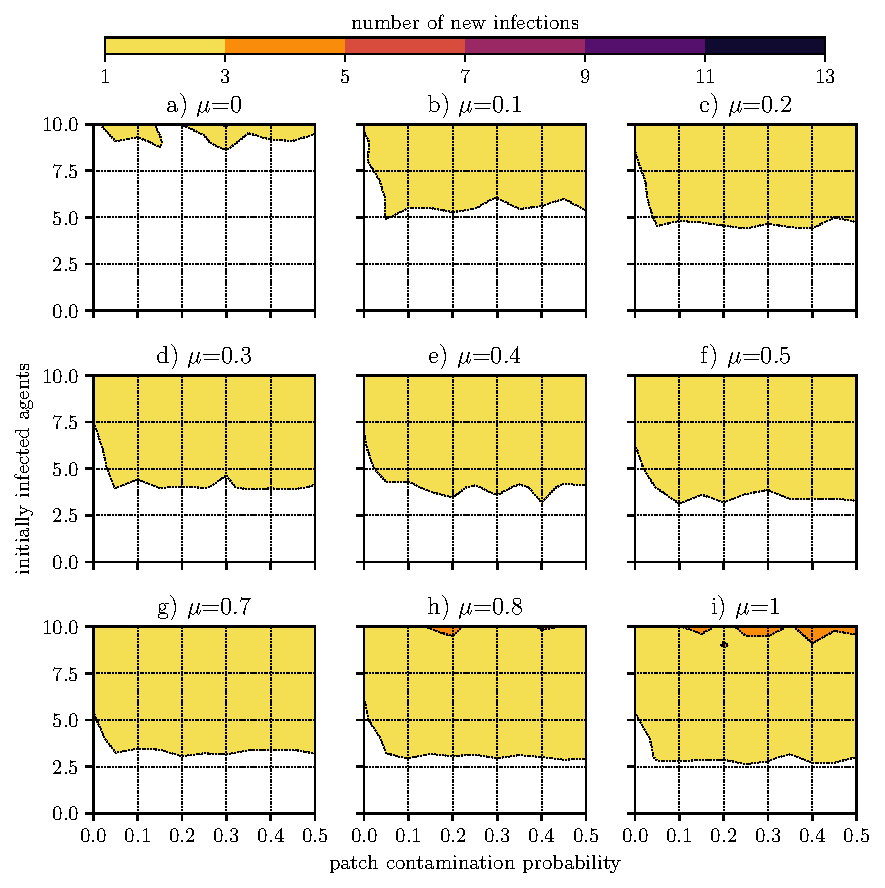
\includegraphics[scale=0.75]{plots/sick_increase_small_s_pop100_world-3.pdf}
\end{center}
\caption{Mean increase in the number of infected agents for different values of mobility parameter $\mu$ with the contamination parameters for the population without coughing agents. The population of agents was set to 100 and configuration of obstacles from Fig~\ref{fig:gui-world-3}. The colour scale is the same as in the Figs~\ref{fig:sick_increase_large_s_pop100} and \ref{fig:sick_increase_large_s_pop50}. One should note that even for the significant portion of the infected agents in the population, the spread of the disease is limited.}
\label{fig:sick_increase_small_s_pop100_world-3}
\end{figure}


\begin{figure}[ht!]
\begin{center}
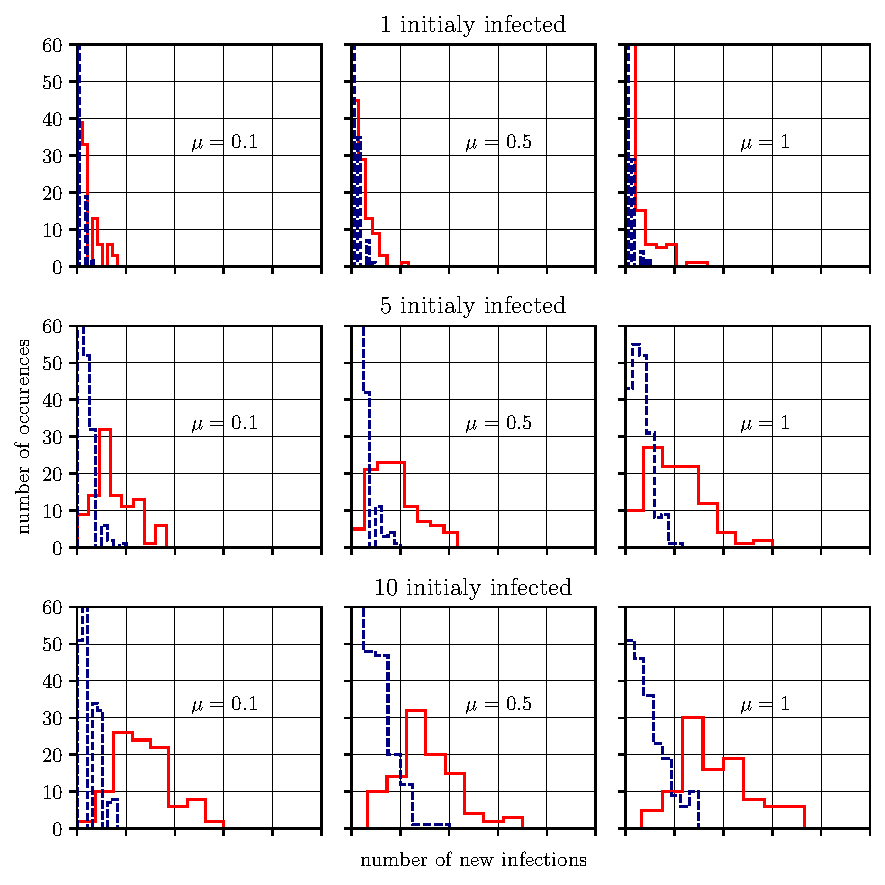
\includegraphics[scale=0.75]{plots/plot_pop100_world-1_exp6_exp7_hist.pdf}
\end{center}
\caption{Dependency between the number of initially infected agents and the mobility. Each row represents series of histograms for a fixed number of initially infected agents (equal to 1, 2, 5 and 10) for changing mobility, for for the case $s=5$ (blue dashed line) and for the case $s=66$ (solid red line). One can observe that for the case when a significant potion og the population is initially infected the changes in the mobility have less prominent impact on the distribution the in the case of small number of initially infected agents. Presented data were generated for \texttt{exp6} and \texttt{exp6} from  \texttt{experiements-v2.xml}.}
\label{fig:exp6_pop100_world-1_hist}
\end{figure}

\begin{thebibliography}{1}
\bibitem{model-src} \url{https://github.com/jmiszczak/indoors_virus_propagation_private}
\end{thebibliography}

\end{document}